%% Relatório do Trabalho 2 de MC714 Sistemas Distribuídos, 2º semestre de 2026.
%% Eleição em Anel, Two-Phase Commit, a integração dos dois e o Bully. Classe IEEEtran, duas colunas.
%% Compilar dentro de docs/relatorio com latexmk -pdf relatorio.tex, ou com pdflatex duas vezes.
%%
%% Os números das tabelas são cópias dos CSVs de docs/dados/ e das tabelas de docs/resultados-*.md,
%% e os dos cenários vêm de results/cenario_*.json. O analisar.py conferir confere só os markdowns,
%% e não este arquivo. Depois de uma bateria ou de um cenário novos, os números daqui mudam à mão.
\documentclass[conference]{IEEEtran}

\usepackage[T1]{fontenc}
\usepackage[utf8]{inputenc}
\usepackage[brazilian]{babel}
\usepackage{amsmath}
\usepackage{graphicx}
\usepackage{booktabs}
\usepackage{array}
\usepackage{tikz}
\usetikzlibrary{babel,positioning,fit,arrows.meta}
\usepackage{url}
\usepackage[hidelinks]{hyperref}

% Figuras versionadas em docs/figuras
\graphicspath{{../figuras/}}

\newcommand{\cod}[1]{\texttt{\upshape #1}}

\begin{document}

\title{Eleição em Anel, Two-Phase Commit e Bully:\\
Correção sob Falhas, Integração e Avaliação}

\author{\IEEEauthorblockN{Pietro Fernandes Magaldi (RA 236842)\qquad
Tiago Perrupato Antunes (RA 194058)}
\IEEEauthorblockA{Instituto de Computação, Universidade Estadual de Campinas (UNICAMP)\\
MC714 Sistemas Distribuídos, 2º semestre de 2026\\[2pt]
Repositório: \url{https://github.com/tiagoperrupato/mc714-t2/tree/entrega-t2}\\
Vídeo: \textbf{[link do vídeo]}}}

\maketitle

\begin{abstract}
Implementamos três algoritmos distribuídos como Nós independentes que trocam HTTP/JSON sobre
Docker Compose: a eleição de Líder em anel, o Two-Phase Commit (2PC) com recuperação do
Coordenador por log durável e a eleição do valentão (Bully). Na integração, o Líder de um anel de
três candidatos coordena o 2PC, e quando ele cai o cliente elege outro, que assume as transações
novas. Declaramos o modelo de cada algoritmo e conferimos nove invariantes de \emph{safety} e
\emph{liveness} sobre os logs dos Nós em 14 cenários, normais e com crash, reinício, partição,
perda e uma falha combinada de Coordenador e Participante. O anel converge com 9,20 Mensagens
para cinco Nós e perda de 0,05, perto das 9,47 previstas. O 2PC custa 12 Mensagens por transação
com três Participantes, e a latência de commit vai de 8,5 a 344,6~ms quando o atraso de ida sobe
de 0 a 50~ms. O Coordenador derrubado depois de decidir se recupera do log em menos de 1~s na
média, com máximo de 1,552~s. Com sete Nós, o Bully gasta 34,60 Mensagens contra 13,40 do anel,
mas converge em 2,60 saltos contra 13,40.
\end{abstract}

\section{Introdução}
\label{sec:intro}
Eleição de Líder e compromisso atômico se completam. O 2PC precisa de um Coordenador, e
escolhê-lo é um problema de eleição. O Coordenador é também o ponto fraco do 2PC: se ele cai
depois de decidir, os Participantes que votaram SIM ficam bloqueados até ele voltar. Este trabalho
implementa os dois lados e mede o custo de cada um. A eleição em anel e o 2PC, apresentados
em~\cite{vansteen}, são os dois algoritmos principais. A integração faz o Líder do anel coordenar
o 2PC e mostra o que uma reeleição resolve e o que não resolve. O Bully, terceiro algoritmo, é a
outra eleição clássica, comparada com o anel nas mesmas condições.

Cada Nó lógico roda num contêiner próprio e só se comunica pela rede. As falhas entram pela
aplicação e pela rede, dirigidas por uma Semente registrada, e cada cenário grava os logs dos Nós,
que um verificador separado confere contra os invariantes.

\section{Arquitetura}
\label{sec:arq}
Um núcleo comum (\cod{src/comum}) oferece configuração validada, modelos imutáveis, streams de
aleatoriedade por Semente, log estruturado em JSON e o Transporte HTTP com Deadline obrigatório.
Cada algoritmo é construído da Máquina de Estados pura para fora (Fig.~\ref{fig:arq}). A Máquina
é um conjunto de funções puras sobre estado imutável, que recebem uma Mensagem ou um prazo e
devolvem o novo estado e o que fazer: as Mensagens a enviar e, no 2PC, as gravações no log, na
ordem write-ahead. Ela nunca importa FastAPI nem httpx. Um adaptador fino (\cod{no.py},
\cod{coordenador.py}, \cod{participante.py} ou \cod{candidato.py}) liga a Máquina à rede e despacha
os envios por uma fila de saída, fora do caminho da resposta HTTP. Assim a mesma lógica roda nos
testes, nas baterias em processo e nos contêineres.

Todos os Nós usam a mesma imagem, e o \cod{command} de cada serviço escolhe o algoritmo. A
topologia vem toda de variáveis de ambiente. O \cod{compose.yaml} sobe o anel de cinco Nós, o 2PC
com um Coordenador e três Participantes, cada um com um volume próprio para o Log Durável, e o
Toxiproxy. A integração e o Bully têm pilhas próprias, \cod{compose.integracao.yaml} e
\cod{compose.bully.yaml}.

\textbf{Integração.} Cada um dos três candidatos roda, no mesmo processo, um Nó do anel e um
Coordenador do 2PC. Um único \cod{POST /mensagem} recebe as Mensagens dos dois algoritmos e
despacha pelo tipo: eleição e anúncio de Líder vão ao Nó do anel, Voto e ACK ao Coordenador. Só o
Líder aceita \cod{POST /transacao}, e os outros respondem 409 com o id do Líder. O Participante
responde à origem da Mensagem quando ela está na lista de Coordenadores conhecidos e recusa as
demais.

\textbf{Bibliotecas.} Python 3.12 com FastAPI 0.162.0 e uvicorn 0.34.0 no servidor, httpx 0.28.1
no cliente, pandas 3.0.2 e matplotlib 3.10.8 na análise, e Toxiproxy 2.9.0 para as falhas de rede.
Nenhuma biblioteca implementa eleição nem commit atômico. FastAPI, uvicorn e httpx só transportam
JSON, o Toxiproxy só atrasa ou corta conexões, e a lógica dos algoritmos está em
\cod{src/anel/maquina.py}, \cod{src/doispc/maquina.py} e \cod{src/bully/maquina.py}.

\begin{figure}[t]
\centering
\begin{tikzpicture}[font=\scriptsize, >=Stealth,
  caixa/.style={draw, rounded corners=1.5pt, align=center, inner sep=2pt},
  camada/.style={caixa, minimum width=3.9cm}]
  \node[caixa, minimum width=8.3cm] (cond) at (4.15,0)
    {condutor (\cod{cenario.py}, \cod{bateria.py}) e testes};
  \node[camada] (app) at (2.05,-1.0) {adaptador FastAPI};
  \node[camada, below=0.6mm of app] (maq) {Máquina de Estados pura};
  \node[camada, below=0.6mm of maq] (comum)
    {núcleo comum: Transporte com\\Deadline, falhas, logs};
  \node[draw, dashed, rounded corners, inner sep=2pt, fit=(app)(maq)(comum)] (no) {};
  \node[anchor=south west, inner sep=1pt] at (no.north west) {Nó (um contêiner)};
  \node[caixa, minimum width=1.7cm, minimum height=1.2cm] (toxi) at (no.east -| 5.55,0)
    {Toxiproxy:\\latência e\\partição};
  \node[caixa, minimum width=1.3cm, minimum height=1.2cm] (outros) at (no.east -| 7.65,0)
    {outros\\Nós};
  \draw[<->] (no.east) -- node[above=1pt, font=\tiny] {HTTP} (toxi.west);
  \draw[<->] (toxi.east) -- (outros.west);
  \draw[->] (3.4,0 |- cond.south) -- node[right, font=\tiny] {controle HTTP} (3.4,0 |- no.north);
  \draw[->] (cond.south -| outros.north) -- (outros.north);
  \node[caixa, minimum width=8.3cm, below=4mm of no.south west, anchor=north west, xshift=-0.07cm]
    (res) {\cod{results/}: logs JSONL e Log Durável dos Nós, CSVs e JSON dos cenários};
  \draw[->] (no.south) -- (res.north -| no.south);
  \draw[->] (outros.south) -- (res.north -| outros.south);
  \node[caixa, minimum width=4.0cm, below=3mm of res.south west, anchor=north west] (ver)
    {\cod{verificar.py}: invariantes 01 a 09};
  \node[caixa, minimum width=4.0cm, below=3mm of res.south east, anchor=north east] (ana)
    {\cod{analisar.py}: tabelas e figuras};
  \draw[->] (res.south -| ver.north) -- (ver.north);
  \draw[->] (res.south -| ana.north) -- (ana.north);
\end{tikzpicture}
\caption{Camadas de um Nó e caminho dos dados. As Mensagens passam pelo Toxiproxy quando o
cenário ou a bateria aplica falha de rede.}
\label{fig:arq}
\end{figure}

\section{Modelo do sistema}
\label{sec:modelo}
A Tabela~\ref{tab:modelo} resume o modelo de cada algoritmo. Três pontos são comuns.

\textbf{Canais (M2).} HTTP/JSON ponto a ponto, não confiáveis. Uma Mensagem pode ser perdida ou
atrasada, e sob partição não é entregue. Um reenvio pode duplicá-la, e não há ordem garantida
entre Mensagens distintas. Toda chamada leva um Deadline obrigatório, porque o cliente não tem
caminho que envie sem timeout, e as falhas de transporte viram resultados tipados (timeout, conexão
recusada, indisponível). É o Deadline que converte ``não chegou'' numa decisão: o salto no anel e o
ABORT por timeout no 2PC.

\textbf{Relógios (M4).} Nenhum algoritmo depende de relógio físico. A correção repousa na ordem
causal de cada Nó e nos Deadlines, e os prazos do Bully são durações medidas no próprio Nó. O
carimbo de tempo do log serve só para lê-lo.

\textbf{Falhas (M3).} Duas camadas, as duas registradas com a Semente. Na aplicação, \cod{/falha/*}
liga crash (o Nó responde 503 e não envia nada), pause, delay e drop, os dois últimos sorteados de
streams da Semente. Na rede, o Toxiproxy aplica latência e partição de entrada ao anel e ao 2PC,
com o override \cod{compose.toxiproxy.yaml}. Neles, todo Nó alcança o destino pelo proxy do
destino, e desativá-lo corta as Mensagens que chegam ao Nó, e não as que ele envia. Isso isola um
Nó do anel ou um Participante, porque eles só enviam em resposta ao que recebem. O Bully e a
integração não passam pelo Toxiproxy. A perda de Mensagens vem do drop da aplicação e das baterias, e não do Toxiproxy. O crash
de processo é o \cod{docker compose kill}, ou a saída do Coordenador logo depois de gravar a
Decisão. A detecção é sempre por timeout e pode errar: um Nó lento é tratado como falho e volta a
ser visto quando os atrasos cabem de novo no prazo, a semântica \emph{fail-noisy}.

\begin{table*}[t]
\caption{Modelo do sistema por algoritmo. M1 a M7 numeram, na ordem, os itens do modelo pedidos no
enunciado.}
\label{tab:modelo}
\centering
\footnotesize
\setlength{\tabcolsep}{3pt}
\renewcommand{\arraystretch}{1.1}
\begin{tabular}{@{}>{\raggedright\arraybackslash}p{1.35cm}
  *{4}{>{\raggedright\arraybackslash}p{3.95cm}}@{}}
\toprule
& \textbf{Anel} & \textbf{2PC} & \textbf{Integração} & \textbf{Bully} \\
\midrule
M1 temporal & Parcialmente síncrono. Deadline de 1~s, com três tentativas de entrega antes do
salto. & Parcialmente síncrono. Prazo de 3~s para os Votos, e um timeout que erra só causa um
ABORT desnecessário. & Herdado dos dois. Sem detector de falha do Líder: o cliente percebe a
queda pelo erro ou pelo prazo do \cod{POST /transacao}. & Síncrono, a hipótese do Bully. Com
D = 1~s, PRAZO\_OK = 2,5~s $>$ 2D e PRAZO\_COORDENADOR = 5~s $>$ PRAZO\_OK + 2D. \\
M2 canais & Unidirecional. Cada Nó fala só com o Sucessor, que aceita com \cod{ack}. & Estrela.
PREPARE e DECISAO descem, VOTO e ACK sobem, e a DECISAO é retransmitida a cada 1~s até o ACK. &
Um \cod{POST /mensagem} por candidato despacha ao Nó do anel ou ao Coordenador. O Participante só
aceita Coordenadores conhecidos. & Todos com todos, com uma fila de saída por destino. O OK é
Mensagem do protocolo, e não a resposta HTTP. \\
M3 falhas & Crash-stop, crash-recovery e partição de entrada do Líder. Suspeita errada de Nó
lento. & Crash-stop e crash-recovery do Coordenador e dos Participantes, partição entre eles e
Participante lento. & Crash-recovery do candidato, que derruba juntos o Nó do anel e o
Coordenador. Participante que descarta tudo. & Crash-stop e crash-recovery de qualquer Nó, perda
de Mensagem e suspeita errada. \\
M4 persistência e reinício & Sem estado durável. O Nó volta sem memória e participa da próxima
eleição pedida. & Log Durável write-ahead com \cod{fsync}. O Coordenador relê o log, difunde o que
estava decidido e aborta o que estava em WAIT. & Log Durável por candidato. O que volta recupera
só as próprias transações e não conhece Líder até a eleição seguinte. & Sem estado durável. O Nó
convoca ao subir e assume na hora se é o maior id, ou no prazo de OK se é só o maior vivo. \\
M5 e M6 & Invariantes 01 a 03 nos logs. & 04 a 07 nos logs, terminação nos cenários. & 01 a 07,
failover nos cenários. & 08 e 09 nos logs. \\
M7 Nós & 5 no compose, 3, 5 e 7 na bateria. Sem o Líder restam 4. & 1 Coordenador e 3
Participantes: o abort tem SIM e NAO, e o crash deixa vários em dúvida. & 3 candidatos e 3
Participantes. Sem o Líder resta um anel de 2. & 5 no compose, 3, 5 e 7 na bateria. Sem o maior
restam 4. \\
\bottomrule
\end{tabular}
\end{table*}

\section{Algoritmos}
\label{sec:algoritmos}

\subsection{Eleição em anel}
Usamos o anel unidirecional com lista acumulada de ids~\cite{vansteen}. Quem inicia abre uma
rodada com id único e envia ao Sucessor a eleição com o próprio id. Cada Nó acrescenta o seu e
repassa. Quem recebe a lista com o próprio id fecha a volta, elege o maior e circula o anúncio do
Líder, que para no primeiro Nó que já conhecia o resultado. Um Nó que já fechou a rodada ignora uma
eleição atrasada dela, que a fecharia de novo com outro Líder. O Nó tenta entregar ao Sucessor até
três vezes dentro do Deadline, uma a cada terço dele, e só então o salta para o próximo vivo. Uma
rodada com um iniciador custa $2n$ Mensagens, e o último Nó conhece o Líder depois de $2n-1$.

A eleição só começa por \cod{POST /iniciar-eleicao}, pedido pelo cenário, pelo teste ou pelo
operador. Nenhum Nó inicia uma rodada sozinho, nem ao suspeitar do Líder. Um Nó que reinicia volta
sem memória, zera as suspeitas ao entrar numa rodada nova e participa da próxima eleição pedida.

\subsection{Two-Phase Commit}
\label{sec:2pc}
O 2PC é bloqueante, com recuperação do Coordenador e retransmissão da DECISAO até o
ACK~\cite{vansteen}. Não há \emph{presumed abort} nem terminação cooperativa, então o bloqueio dura
enquanto o Coordenador está fora. O Coordenador grava a entrada em WAIT, envia os PREPARE e coleta
os Votos até o prazo. Com todos SIM decide COMMIT, e com um NAO ou com o prazo estourado decide
ABORT. Ele grava a Decisão antes de difundi-la e a retransmite a cada Participante até o ACK, uma
Mensagem do protocolo enviada depois de gravar e aplicar. O Participante grava o Voto antes de
respondê-lo e a Decisão antes de aplicá-la, e cada entrada recebe \cod{fsync} antes do efeito que
depende dela. Cada transação tem um id, e um \cod{POST /transacao} com id já usado devolve a
Decisão ou espera a rodada em curso, então o cliente pode repetir o pedido sem risco. Na partida, o
Coordenador relê o log, difunde de novo o que estava decidido e aborta o que estava em WAIT, porque
não guardou os Votos. Sem falha, uma transação custa $4N$ Mensagens com $N$ Participantes: PREPARE,
VOTO e DECISAO somam $3N$, e o ACK é a Mensagem a mais que a retransmissão exige.

O Deadline e o write-ahead não são detalhe de estilo. Sem o Deadline obrigatório, uma partição
entre o Coordenador e um Participante travaria a coleta de Votos, o ABORT por timeout nunca ocorreria e a transação não
terminaria. O cenário \cod{2pc particao} mostra o ABORT no prazo. Se a gravação da Decisão migrasse
para depois da resposta de rede, um crash entre responder e gravar perderia a Decisão, e o
invariante 05 reprovaria a reversão. Sem a entrada em WAIT, um Coordenador que cai antes de decidir
voltaria sem saber que a transação existiu, e os Participantes que votaram SIM ficariam em dúvida
para sempre.

\section{Propriedades de correção}
\label{sec:props}
A Tabela~\ref{tab:props} liga cada propriedade (M5) ao invariante que a confere sobre os logs dos
Nós (M6), em \cod{src/analise/invariantes.py}. Cada invariante tem três desfechos: passa, reprova
ou lacuna, quando o log não tem o caso que ele confere. Só a reprovação muda o código de saída. A
tolerância é zero em todos, porque são igualdades entre inteiros ou rótulos, sem variância a
absorver.

O Participante que votou SIM e não tem Decisão durável está em dúvida. O invariante 05 o registra
como aviso, e não como reprovação, porque esse bloqueio é o preço da atomicidade sem terminação
cooperativa. A terminação do 2PC fica nos cenários, que sabem qual falha injetaram e saem 1 quando
o desfecho difere do esperado.

Com a detecção que erra, o anel não garante a unicidade em toda execução. Se o 4 suspeita por
engano do 5, que está lento, e do 1, ele salta os dois, e a mesma rodada pode fechar duas vezes,
como reproduz um teste. Por isso o 01 é conferido em cada execução.

\begin{table}[t]
\caption{Propriedades de correção e como são verificadas.}
\label{tab:props}
\centering
\footnotesize
\setlength{\tabcolsep}{4pt}
\begin{tabular}{@{}l>{\raggedright\arraybackslash}p{4.95cm}>{\raggedright\arraybackslash}p{1.1cm}@{}}
\toprule
Inv. & Propriedade & Tipo \\
\midrule
\multicolumn{3}{@{}l}{\emph{Eleição em anel}} \\
01 & No máximo um Líder por rodada concluída & safety \\
02 & Todos os vivos convergem ao mesmo Líder & safety e liveness \\
03 & O Líder é o maior id vivo, descontados os saltados na rodada & safety \\
\multicolumn{3}{@{}l}{\emph{Two-Phase Commit}} \\
04 & Atomicidade: nenhum COMMIT com outro ABORT na mesma transação & safety \\
05 & Durabilidade: a Decisão relida no reinício é a gravada & safety \\
06 & Validade: COMMIT só com o Voto SIM de todos os Participantes & safety \\
07 & Coordenador único por transação, mesmo com dois Líderes na integração & safety \\
cen. & Terminação: todo Participante decide, em 10~s sem falha e em 30~s depois que o
Coordenador volta & liveness \\
aviso & Participante em dúvida enquanto o Coordenador está fora & bloqueio \\
\multicolumn{3}{@{}l}{\emph{Integração}} \\
cen. & Transações novas voltam a comitar depois da reeleição, em 10~s & liveness \\
\multicolumn{3}{@{}l}{\emph{Bully}} \\
08 & Nenhum Nó aceita Líder de id menor que o seu & safety \\
09 & Ao fim, todo vivo tem como Líder o maior id vivo, em até 30~s & liveness \\
\bottomrule
\end{tabular}
\end{table}

\section{Testes e verificação}
\label{sec:testes}
A suíte \cod{pytest} tem uma parte sem Docker e uma parte marcada \cod{slow}, que sobe o compose,
e as duas passam na versão entregue. A primeira cobre as Máquinas de Estados, o Transporte, as falhas, as baterias, a análise e os
invariantes. Entre eles
estão a pausa do Nó 5 numa eleição sem gerar dois Líderes, o Coordenador reiniciado em WAIT que aborta, a DECISAO perdida que chega pela
retransmissão, dois candidatos da integração que se julgam Líderes
e comitam dez transações sem que 04, 06 e 07 reprovem, e uma propriedade do Bully sob escalonamento
sorteado, com perda, duplicata, queda e retorno, em 500 Sementes. Os testes com Docker rodam
cenários de ponta a ponta, a partição do Líder do anel pelo Toxiproxy, uma Réplica curta de
cada bateria do 2PC e um ciclo de construção, subida e remoção sem contêineres órfãos.

A verificação é separada da execução. O \cod{verificar.py} aplica os nove invariantes a cada
diretório de logs de \cod{results/}. Cada cenário declara os invariantes que demonstra, e uma
lacuna num deles o reprova, então um cenário sem log não passa. Os logs e o JSON de cada cenário são
versionados, e o \cod{analisar.py conferir} sai 1 se uma tabela dos documentos divergir dos CSVs.

\section{Cenários, métricas e ambiente}
\label{sec:metodo}
A correção e o desempenho são avaliados à parte. A correção sai dos 14 cenários sobre o compose da
Tabela~\ref{tab:cenarios}, cada um com a Semente 0. O desempenho sai de três baterias.

\textbf{Anel e Bully.} As duas baterias rodam em processo sobre as Máquinas de Estados, nas mesmas
condições: $n$ de 3, 5 e 7 Nós, todos vivos, o Nó 1 como único iniciador, perda de 0,05 por
tentativa de entrega, sorteada do stream \cod{drop} da Semente, reenvio até a entrega e cinco
Réplicas por nível, com as Sementes de 42 a 56. As métricas são as Mensagens, contando toda
tentativa, e o tempo em saltos lógicos, a maior profundidade causal em que um Nó passa a aceitar o
maior id, com um salto a mais por tentativa perdida. No anel há uma Mensagem em trânsito por vez, e
os passos de entrega são esses saltos. Essas métricas se repetem dígito a dígito com a mesma Semente
e se comparam direto com a complexidade, o que
segundos de relógio numa só máquina não permitem.

\textbf{2PC.} A bateria mede os Nós reais no compose, um Coordenador e três Participantes votando
SIM, com o Toxiproxy aplicando atraso de ida de 0, 10, 25 e 50~ms, sem jitter, nos dois sentidos de
cada proxy. Cada Réplica sobe a pilha do zero e roda 45 transações em sequência, das quais as 5
primeiras são aquecimento descartado, e cada transação só começa depois dos ACK da anterior. São
cinco Réplicas por nível, com as Sementes de 42 a 61. A latência de commit vai do
\cod{POST /transacao} à resposta, que sai com a Decisão já no log. Ela entra com a média e o IC 95\%
das médias das Réplicas e com os percentis de todas as transações do nível. As Mensagens de uma
transação são os eventos \cod{envia} dela nos logs de todos os Nós. Na recuperação, com as Sementes
de 62 a 81, cada Réplica derruba o Coordenador logo depois de gravar a Decisão, e o tempo vai do
\cod{docker compose start} até os três Participantes reportarem a Decisão.

\textbf{Ambiente.} Baterias e cenários rodaram num Apple M2 com 8 CPUs e 8 GB de memória, em macOS
26.7.3 (Darwin 25.6.0, arm64). Os contêineres rodam na VM Linux do Docker Desktop (kernel
7.0.14-linuxkit, 8 CPUs e cerca de 4 GB), com Docker 29.9.3, Compose 5.7.0 e Toxiproxy 2.9.0. O
Python é o 3.12.13 no hospedeiro e o 3.12.16 na imagem \cod{python:3.12-slim}. Cada linha dos CSVs e cada JSON de cenário carimba o ambiente. As
baterias do anel e do Bully levam menos de um segundo e não têm aquecimento, porque a métrica é
lógica. A do 2PC leva cerca de 10~min, e as 45 transações de uma Réplica levam de 1,050~s, sem
atraso, a 30,667~s, com 50~ms. Os prazos do compose estão na Tabela~\ref{tab:modelo}, mais 2~s por
envio do 2PC.

\section{Resultados}
\label{sec:resultados}

\subsection{Eleição em anel}
Com perda $p$, cada entrega custa em média $1/(1-p)$ tentativas, e o esperado é $(2n-1)/(1-p)$
(Tabela~\ref{tab:anel}). Em $n=3$ nenhuma tentativa se perdeu nas cinco Réplicas, e o valor fica
exatamente em $2n-1$. Em $n=5$ e $n=7$ o esperado com perda cai dentro do IC 95\%. O custo cresce
linearmente com $n$. Com $k$ iniciadores, o custo sobe para até $k\cdot 2n$, caso que a bateria
não mede.

\begin{table}[t]
\caption{Mensagens até a convergência do anel, com perda de 0,05 e cinco Réplicas por nível,
todas convergidas. Fonte: \cod{analisar.py anel-complexidade}.}
\label{tab:anel}
\centering
\footnotesize
\begin{tabular}{@{}rrrrr@{}}
\toprule
$n$ & Mensagens & IC 95\% ($\pm$) & $2n-1$ & $(2n-1)/(1-p)$ \\
\midrule
3 & 5,00  & 0,00 & 5  & 5,26  \\
5 & 9,20  & 0,56 & 9  & 9,47  \\
7 & 13,40 & 0,68 & 13 & 13,68 \\
\bottomrule
\end{tabular}
\end{table}

\subsection{Latência e Mensagens do 2PC}
As Mensagens ficam em 12,00 por transação em todos os níveis, igual a $4N$, sem nenhuma
retransmissão. A latência cresce em linha com o atraso (Tabela~\ref{tab:2pc-lat}). O Coordenador envia os PREPARE em sequência, e cada envio espera a resposta
do Participante. O último PREPARE sai depois de $N-1$ idas e voltas, e ele e o Voto somam mais duas
idas: $2N=6$ atrasos de ida no caminho crítico. Sobre o piso de 8,5~ms medido sem atraso, o
acréscimo é de 74,8, 181,3 e 336,1~ms para 60, 150 e 300~ms previstos, razões de 1,25, 1,21 e 1,12.
O excesso vem do \cod{fsync} do Voto, do repasse pelo Toxiproxy e do despacho pela fila de saída de
cada Nó. Com os PREPARE em paralelo, o caminho crítico ficaria em dois atrasos de ida para
qualquer $N$.

\begin{table}[t]
\caption{Latência de commit do 2PC, em ms, por atraso de ida, com 200 transações medidas por
nível. A última coluna divide o acréscimo sobre 0~ms por $2N\times$atraso. Fonte:
\cod{analisar.py 2pc-latencia} e \cod{2pc-complexidade}.}
\label{tab:2pc-lat}
\centering
\footnotesize
\setlength{\tabcolsep}{4pt}
\begin{tabular}{@{}rrrrrrr@{}}
\toprule
Rede & Média & IC 95\% ($\pm$) & p50 & p95 & p99 & Razão \\
\midrule
0  & 8,5   & 2,1 & 7,1   & 13,0  & 29,3  & n/d  \\
10 & 83,3  & 0,5 & 83,7  & 90,9  & 105,3 & 1,25 \\
25 & 189,8 & 4,4 & 189,1 & 210,4 & 245,1 & 1,21 \\
50 & 344,6 & 2,1 & 345,0 & 363,7 & 371,7 & 1,12 \\
\bottomrule
\end{tabular}
\end{table}

\subsection{Recuperação do Coordenador}
Na Tabela~\ref{tab:2pc-rec}, a média fica abaixo de 1~s em todos os níveis, mas o máximo não: chega
a 1,262~s com 10~ms e a 1,552~s com 25~ms. A maior parte do tempo, e quase toda a variação entre
Réplicas, vem da partida do contêiner e do interpretador, como mostram os logs da bateria, que
ficam fora do git. As Mensagens passam de 12
porque o Coordenador difunde a Decisão relida antes de o servidor HTTP dele aceitar conexões. Os
ACK que chegam nessa janela falham, e a retransmissão de 1~s repete a DECISAO e o ACK desses
Participantes. Com mais atraso, menos ACK chegam cedo demais, e a contagem cai de 18,00 para 14,00.

\begin{table}[t]
\caption{Tempo de recuperação do 2PC após o crash do Coordenador, por atraso de ida, com cinco
Réplicas por nível. Fonte: \cod{analisar.py 2pc-recuperacao}.}
\label{tab:2pc-rec}
\centering
\footnotesize
\setlength{\tabcolsep}{4pt}
\begin{tabular}{@{}rrrrrr@{}}
\toprule
Rede (ms) & Média (s) & IC 95\% ($\pm$) & Mín.\ (s) & Máx.\ (s) & Mensagens \\
\midrule
0  & 0,553 & 0,030 & 0,533 & 0,592 & 18,00 \\
10 & 0,787 & 0,349 & 0,590 & 1,262 & 18,00 \\
25 & 0,866 & 0,477 & 0,671 & 1,552 & 16,80 \\
50 & 0,817 & 0,048 & 0,789 & 0,884 & 14,00 \\
\bottomrule
\end{tabular}
\end{table}

\begin{table*}[t]
\caption{Cenários sobre o compose. Em todos, a verificação sai com código 0, o desfecho observado
é o esperado e nenhum invariante exigido fica em lacuna. Os tempos vêm de
\cod{results/cenario\_*.json}.}
\label{tab:cenarios}
\centering
\footnotesize
\setlength{\tabcolsep}{4pt}
\begin{tabular}{@{}>{\raggedright\arraybackslash}p{3.45cm}>{\raggedright\arraybackslash}p{3.95cm}
  >{\raggedright\arraybackslash}p{7.75cm}l@{}}
\toprule
Cenário & Falha injetada & Desfecho observado & Passam \\
\midrule
\cod{anel normal} & nenhuma & os cinco elegem o 5, em 0,1372~s & 01 a 03 \\
\cod{anel falha} & kill do 5 após a eleição & os quatro vivos reelegem o 4, em 0,7011~s & 01 a 03 \\
\cod{anel reinicio} & como o anterior, e start do 5 & o 5 volta sem Líder e sem rodadas e não
inicia eleição, e só a terceira, pedida pelo condutor, o reintegra, em 0,0269~s & 01 a 03 \\
\cod{2pc commit} & nenhuma & COMMIT nos três Participantes, em 0,0533~s & 04, 06, 07 \\
\cod{2pc abort} & o 13 vota NAO & ABORT nos três, em 0,0957~s & 04, 07 \\
\cod{2pc crash-coord} & Coordenador cai depois de gravar o COMMIT & três em dúvida e três avisos
com ele fora, COMMIT nos três 1,369~s depois do reinício & 04 a 07 \\
\cod{2pc crash-coord-part} & como o anterior, e o 11 cai e volta em dúvida e depois de decidir &
COMMIT nos três 0,552~s depois do reinício, e o 05 confere duas recuperações & 04 a 07 \\
\cod{2pc particao} & proxy do 11 desativado até o ABORT & ABORT em 3,0164~s, o 11 sem Decisão até a
cura, e ABORT nele pela retransmissão & 04, 07 \\
\cod{integracao normal} & nenhuma & o 1 responde 409, e o Líder 3 comita \cod{c3-tx-n} em 0,0385~s &
01 a 04, 06, 07 \\
\cod{integracao failover} & o 3 cai depois de gravar o COMMIT de \cod{c3-tx-a} & o 2 é eleito e
comita \cod{c2-tx-b}, e \cod{c3-tx-a} termina em COMMIT quando o 3 volta
(Tabela~\ref{tab:failover}) & 01 a 07 \\
\cod{integracao}\newline\cod{failover-isolamento} & como o anterior, e o 11 descarta tudo (drop com $p=1$)
durante \cod{c2-tx-b} & \cod{c2-tx-b} aborta em 3,034~s, o ABORT chega ao 11 depois da limpeza, e
\cod{c3-tx-a} termina em COMMIT & 01 a 07 \\
\cod{bully normal} & nenhuma & a eleição pedida ao 1 termina no OK do 5, em 0,0296~s & 08, 09 \\
\cod{bully falha} & kill do 5 & a eleição pedida ao 1 elege o 4, em 2,5283~s & 08, 09 \\
\cod{bully retorno} & como o anterior, e start do 5 & o 5 assume sem eleição pedida, e os cinco
o seguem 0,7365~s após o start & 08, 09 \\
\bottomrule
\end{tabular}
\end{table*}

\subsection{Correção sob falha}
A Tabela~\ref{tab:cenarios} resume os 14 cenários. No \cod{anel falha}, quase todo o tempo de
reeleição são as três tentativas do 4 de entregar ao 5 morto, antes do salto. No
\cod{2pc crash-coord}, a verificação feita com o Coordenador fora dá o aviso de dúvida dos três
Participantes e sai 0, porque o bloqueio é esperado. Depois do reinício o aviso some, e o 05
confere a Decisão recuperada do log contra a gravada. No \cod{2pc particao}, o ABORT sai no prazo
de 3~s da coleta de Votos.

\section{Conceitos adicionais}
\label{sec:extras}

\subsection{Falha combinada: Coordenador e Participante}
O \cod{2pc crash-coord-part} junta duas falhas. O Coordenador cai logo depois de gravar o COMMIT, e
os três Participantes ficam em dúvida. Com ele fora, o contêiner do Participante 11 cai e volta,
relê o próprio log e reporta Voto SIM, sem Decisão e em dúvida. A verificação feita nesse ponto dá
os três avisos e nenhuma reprovação. O Coordenador volta, relê o log e difunde o COMMIT, e os três
decidem em 0,552~s. Por fim o 11 cai e volta de novo, agora com Voto SIM e COMMIT. A segunda
recuperação do 11 é o caso de Participante do invariante 05, ao lado da do Coordenador, e as duas
reproduzem a Decisão gravada. Os invariantes 04 a 07 passam.

\subsection{Integração: o Líder do anel coordena o 2PC}
O problema é um serviço de transações atômicas sobre três Participantes, com três candidatos a
Coordenador no anel $1\to2\to3\to1$ (Seção~\ref{sec:arq}). O Líder aceita as transações, e quando
ele cai outro candidato assume as novas. Cada transação leva no id o prefixo do candidato que a
criou, como \cod{c3-tx-a}, e só ele a coordena. Se o Deadline do anel suspeita de um candidato vivo
e dois se julgam Líderes, cada transação continua com um só Coordenador, o que o invariante 07
confere. Nenhum candidato assume a transação de outro: só o log do 3 sabe se ele gravou o COMMIT de
\cod{c3-tx-a}, e abortá-la no lugar dele violaria a atomicidade.

A Tabela~\ref{tab:failover} traz a linha do tempo do \cod{integracao failover}. O failover, do erro
de \cod{c3-tx-a} à resposta de \cod{c2-tx-b}, leva 0,7319~s, quase todo na reeleição. No
\cod{failover-isolamento}, o 11 descarta o PREPARE de \cod{c2-tx-b}, o 2 decide ABORT no prazo de
Votos e o failover leva 3,745~s. Depois da limpeza, a retransmissão leva o ABORT ao 11, que grava a
Decisão sem Voto.

\begin{table}[t]
\caption{Linha do tempo do \cod{integracao failover}. Fonte:
\cod{results/cenario\_integracao\_failover.json}.}
\label{tab:failover}
\centering
\footnotesize
\setlength{\tabcolsep}{4pt}
\begin{tabular}{@{}>{\raggedright\arraybackslash}p{6.6cm}r@{}}
\toprule
Etapa & Tempo (s) \\
\midrule
Eleição inicial: os três candidatos têm o 3 como Líder & 0,0761 \\
O 3 grava o COMMIT de \cod{c3-tx-a} e cai: 11, 12 e 13 em dúvida & n/d \\
O cliente vê o erro e pede eleição: os candidatos 1 e 2 têm o 2 como Líder & 0,7018 \\
O 2 comita \cod{c2-tx-b} nos três, com \cod{c3-tx-a} em dúvida neles & 0,0255 \\
O 3 volta, relê o log e difunde o COMMIT de \cod{c3-tx-a} aos três & 0,5468 \\
A eleição seguinte devolve a liderança ao 3 & 0,0243 \\
\bottomrule
\end{tabular}
\end{table}

\subsection{Terceiro algoritmo: Bully}
Implementamos a eleição do valentão de Garcia-Molina~\cite{garciamolina}, também apresentada
em~\cite{vansteen}. Quem convoca manda ELEICAO a cada id maior. Cada maior responde OK e convoca
também, e quem não recebe OK no prazo assume e manda COORDENADOR a todos. A Máquina de Estados
recebe os prazos como eventos e não conhece relógio. Cada convocação abre uma época, que vai na
ELEICAO, no OK e no prazo. Um OK sem Líder ou um prazo de época velha é ignorado, e o OK que traz
Líder maior vale em qualquer época. Todo Nó convoca ao subir, e só o maior id assume na hora. Duas
regras separam a variante da clássica:
\begin{itemize}
\item \emph{O OK leva o Líder em exercício.} O Líder ocioso que recebe ELEICAO de um menor responde
só OK, com o próprio id, e quem recebe esse OK o aceita, salvo se já está ocioso com um Líder maior
ou igual, caso em que o OK é atrasado e é ignorado. Na clássica ele reabre a eleição a cada
ELEICAO atrasada, e numa entrega FIFO o pior caso passa de $n^2-1$ para $n^2-1+(n-1)(n-2)$
Mensagens. Com a regra, ele fica em $n^2-1$ exato.
\item \emph{Um COORDENADOR de id menor é rejeitado.} Quem o recebe convoca, e o menor que assumiu
por suspeita errada perde a liderança para o maior vivo sem esperar outro pedido de eleição.
\end{itemize}
Com as duas regras, o invariante 08 vale em toda execução, inclusive com suspeita errada.

Com o Nó 1 como iniciador, cada Nó $i$ manda ELEICAO aos $n-i$ maiores, e cada uma recebe OK. São
$n(n-1)/2$ de cada, mais os $n-1$ COORDENADOR, ou $n^2-1$ ao todo. Se o maior convoca, são $n-1$.
A Tabela~\ref{tab:bully} conta
até não restar Mensagem em trânsito. Em $n=3$ nenhuma tentativa se perdeu, e o total fica em
$n^2-1$. Em $n=5$ e $n=7$ o esperado com perda cai dentro do IC 95\%.

\begin{table}[t]
\caption{Mensagens do Bully até não restar Mensagem em trânsito, com perda de 0,05 e o Nó 1 como
iniciador. Fonte: \cod{analisar.py bully}.}
\label{tab:bully}
\centering
\footnotesize
\begin{tabular}{@{}rrrrrr@{}}
\toprule
$n$ & Mensagens & IC 95\% ($\pm$) & $n-1$ & $n^2-1$ & $(n^2-1)/(1-p)$ \\
\midrule
3 & 8,00  & 0,00 & 2 & 8  & 8,42  \\
5 & 25,60 & 1,88 & 4 & 24 & 25,26 \\
7 & 51,00 & 1,52 & 6 & 48 & 50,53 \\
\bottomrule
\end{tabular}
\end{table}

A Tabela~\ref{tab:bully-anel} e a Fig.~\ref{fig:bully-anel} comparam os dois algoritmos até o
último Nó aceitar o maior id. Em Mensagens, o anel fica perto de $2n-1$ e o Bully cresce com $n^2$.
Em saltos a relação se inverte. Sem perda, o Bully converge em 2 saltos para todo $n$, porque a
ELEICAO do 1 chega ao maior num salto e o COORDENADOR dele chega a todos no seguinte. Cada tentativa
perdida nesse caminho soma um salto, e por isso a média passa um pouco de 2 em $n=5$ e $n=7$. O
anel precisa de $2n-1$. O Bully paga Mensagens para convergir em tempo que não cresce com $n$.

\begin{table}[t]
\caption{Anel e Bully nas mesmas condições, até o último Nó aceitar o maior id, com média
$\pm$ IC 95\%. As cinco Réplicas convergiram em todos os níveis. Fonte:
\cod{analisar.py bully-anel}.}
\label{tab:bully-anel}
\centering
\footnotesize
\setlength{\tabcolsep}{4pt}
\begin{tabular}{@{}rrrrr@{}}
\toprule
& \multicolumn{2}{c}{Mensagens} & \multicolumn{2}{c}{Saltos} \\
\cmidrule(lr){2-3}\cmidrule(l){4-5}
$n$ & Anel & Bully & Anel & Bully \\
\midrule
3 & 5,00 $\pm$ 0,00  & 7,00 $\pm$ 0,00  & 5,00 $\pm$ 0,00  & 2,00 $\pm$ 0,00 \\
5 & 9,20 $\pm$ 0,56  & 19,00 $\pm$ 1,76 & 9,20 $\pm$ 0,56  & 2,20 $\pm$ 0,56 \\
7 & 13,40 $\pm$ 0,68 & 34,60 $\pm$ 1,67 & 13,40 $\pm$ 0,68 & 2,60 $\pm$ 0,68 \\
\bottomrule
\end{tabular}
\end{table}

\begin{figure}[t]
\centering
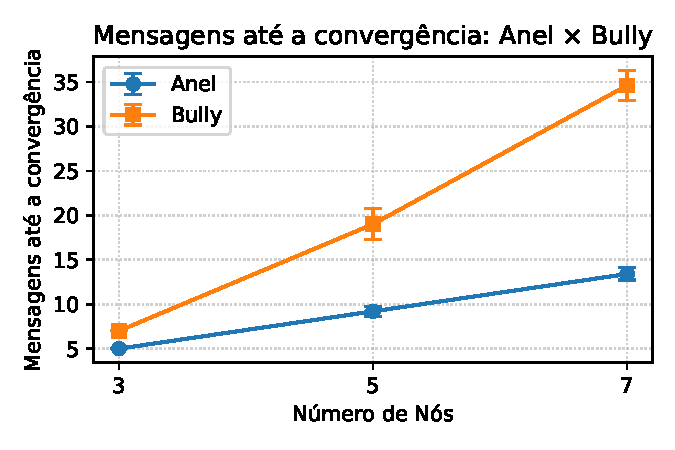
\includegraphics[width=0.92\columnwidth]{anel_bully.pdf}
\caption{Mensagens até a convergência por número de Nós, anel e Bully, com o IC 95\%. Fonte:
\cod{analisar.py bully-anel}.}
\label{fig:bully-anel}
\end{figure}

No \cod{bully falha}, a reeleição leva pouco mais que o PRAZO\_OK de 2,5~s que o 4 espera do 5
morto.

\section{Limitações}
\label{sec:limitacoes}
\textbf{Ambiente.} Os contêineres compartilham kernel, relógio, escalonador e memória de uma só
máquina. São Nós lógicos, e não domínios de falha independentes. Uma partição é um proxy
desativado, e um crash é a morte do processo, e não a queda de um host. Por isso os tempos absolutos
só se comparam entre níveis na mesma máquina. As
propriedades de correção são sobre a ordem lógica dos eventos, que a emulação preserva. Cada
cenário rodou uma vez, e os tempos dele são uma amostra só.

\textbf{Eleições.} As baterias do anel e do Bully rodam em processo, com um só iniciador, e os
contêineres só demonstram a correção. Nenhum Nó inicia eleição sozinho, e o Bully garante o 08 e
o 09 só sob a hipótese síncrona.

\textbf{2PC.} O 2PC é bloqueante: sem terminação cooperativa, um Participante em dúvida só decide
quando o Coordenador volta. A durabilidade vale só contra crash de processo, porque o diretório do log
não recebe \cod{fsync} quando o arquivo é criado, e perder uma entrada já gravada exigiria a queda
do sistema operacional. Os PREPARE em sequência fazem a latência crescer com $N$, e a bateria
mede um só $N$, com todos votando SIM.

\textbf{Integração.} Não há detector de falha do Líder: quem percebe a queda é o cliente, pelo erro
ou pelo prazo do \cod{POST /transacao}, e é ele que pede a eleição. A transação em dúvida espera o
Coordenador dela voltar, o bloqueio do 2PC. E não há
dados nem travas. Num banco, \cod{c2-tx-b} esperaria as travas que \cod{c3-tx-a} segura nos itens
em comum. Aqui ela comita com \cod{c3-tx-a} em dúvida porque nada liga as duas.

\section{Conclusões}
\label{sec:conclusao}
Os três algoritmos e a integração rodam como Nós reais, e nenhum dos nove invariantes reprova nos
logs dos 14 cenários. O anel e o Bully gastam as Mensagens previstas pela complexidade. O 2PC custa $4N$ Mensagens, a latência segue os $2N$ atrasos de ida, e as
propriedades valem com o Coordenador derrubado, também junto com um Participante. A integração
mostra o limite da reeleição: o novo Líder destrava as transações novas, e a que estava em dúvida
espera o Coordenador dela.

% As referências começam numa página própria, fora das seis do corpo.
\clearpage
\begin{thebibliography}{1}
\bibitem{vansteen}
M. van Steen and A. S. Tanenbaum, \emph{Distributed Systems}, 4th ed.
distributed-systems.net, 2023.

\bibitem{garciamolina}
H. Garcia-Molina, ``Elections in a distributed computing system,'' \emph{IEEE Trans.\
Computers}, vol. C-31, no. 1, pp. 48--59, 1982.
\end{thebibliography}

\end{document}
